
\section{Continuidade em $\mathbb R^n$}
Como acontece no caso unidimensional, intuitivamente, uma função $f$ é contínua em um ponto $p$ de seu domínio se, e somente se $f(x)$ fica tão próximo de $f(p)$ quanto se queira, desde que $x$ esteja suficientemente próximo de $p$.

Formalmente, temos a definição abaixo.

\begin{definition}
    Seja $A\subseteq \mathbb R^n$ um conjunto e $f: A \to \mathbb R^m$ uma função.

    Seja $a \in A$. Dizemos que $f$ é contínua em $a$ se, para toda bola aberta $B$ em torno de $f(p)$, existe uma bola aberta $B'$ em torno de $p$ tal que $f[B'\cap A]\subseteq B$.

    Equivalentemente, $f$ é contínua em $p$ se, para todo $\varepsilon > 0$, existe $\delta > 0$ tal que $f[B(p, \delta)\cap A]\subseteq B(f(p), \varepsilon)$.

    Ou, ainda, $f$ é contínua em $p$ se, para todo $\varepsilon > 0$, existe $\delta > 0$ tal que, para todo $x \in A$, se $d(x, p) < \delta$, então $d(f(x), f(p)) < \varepsilon$.

    Dizemos que $f$ é \emph{contínua} se, e somente se, $f$ é contínua em todo ponto de seu domínio $A$.
    \begin{figure}[ht]
        \centering
        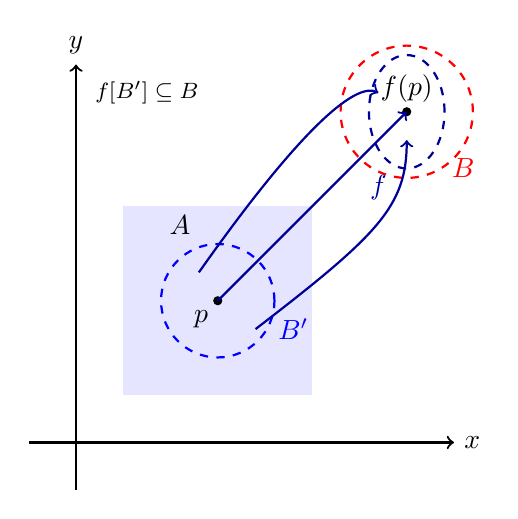
\begin{tikzpicture}[scale=1.2]
            % Eixos
            \draw[->,thick] (-0.5,0) -- (4,0) node[right] {$x$};
            \draw[->,thick] (0,-0.5) -- (0,4) node[above] {$y$};

            % Domínio A
            \draw[fill=blue!10,draw=none] (0.5,0.5) rectangle (2.5,2.5);
            \node at (1.1,2.3) {$A$};

            % Ponto p
            \filldraw[black] (1.5,1.5) circle (1.2pt) node[below left] {$p$};

            % Bola aberta B' em torno de p
            \draw[blue,thick,dashed] (1.5,1.5) circle (0.6);
            \node[blue] at (2.3,1.2) {$B'$};



            % Imagem f(p)
            \filldraw[black] (3.5,3.5) circle (1.2pt) node[above] {$f(p)$};

            % Bola aberta B em torno de f(p)
            \draw[red,thick,dashed] (3.5,3.5) circle (0.7);
            \node[red] at (4.1,2.9) {$B$};

            % Imagem da bola B'
            \draw[->,thick,blue!60!black] (1.3,1.8) .. controls (2.5,3.5) and (3,3.8) .. (3.2,3.7);
            \draw[->,thick,blue!60!black] (1.5,1.5) -- (3.5,3.5);
            \draw[->,thick,blue!60!black] (1.9,1.2) .. controls (3.2,2.2) and (3.5,2.5) .. (3.5,3.2);
            \node[thick,blue!60!black] at (3.2,2.7) {$f$};
            \draw[blue!60!black,thick,dashed] (3.5,3.5) ellipse (.4cm and .6cm);
            % Legenda
            \node[align=left,anchor=west] at (0.1,3.7) {\footnotesize $f[B'] \subseteq B$};
        \end{tikzpicture}
        \caption{Ilustração da continuidade: para toda bola $B$ em torno de $f(p)$, existe uma bola $B'$ em torno de $p$ tal que $f[B'] \subseteq B$.}
    \end{figure}
\end{definition}